\section{Method}
\label{sec:method}

\subsection{Overview}

The design follows from one observation: the unit that must be hidden and the unit that
carries the answer are the same record. Any operation applied to that record therefore has
to do two things at once---keep it addressable, and stop it from stating the value---and none
of the operations a compressor normally has does both. The rule below adds one that does, and
routes every other unit to the cheapest operation that applies.

Given an excerpt $C$, a question $q$, a budget ratio $r$, and the set $V$ of protected
values, \textsc{DARK} produces a rewritten question $q'$ and a compressed context $P$
such that $(q',P)$ fits the token budget and contains no value of $V$. The pipeline has four
steps: split $C$ into units; label each unit on sensitivity and on relevance; apply the
operation attached to its cell; and fit the surviving units into the budget, applying the
alias map to the question at the end. The four operations give the method its name:
\textbf{D}elete, \textbf{A}lias, \textbf{R}efill and \textbf{K}eep.
Algorithm~\ref{alg:dark} states the procedure.
There is no training and no model access at this stage. The only deployment-specific input
is $V$, which an operator already holds for redaction. Figure~\ref{fig:pipeline} shows the
pipeline end to end and the evidence for its one non-obvious choice.

\begin{figure*}[t]
\centering
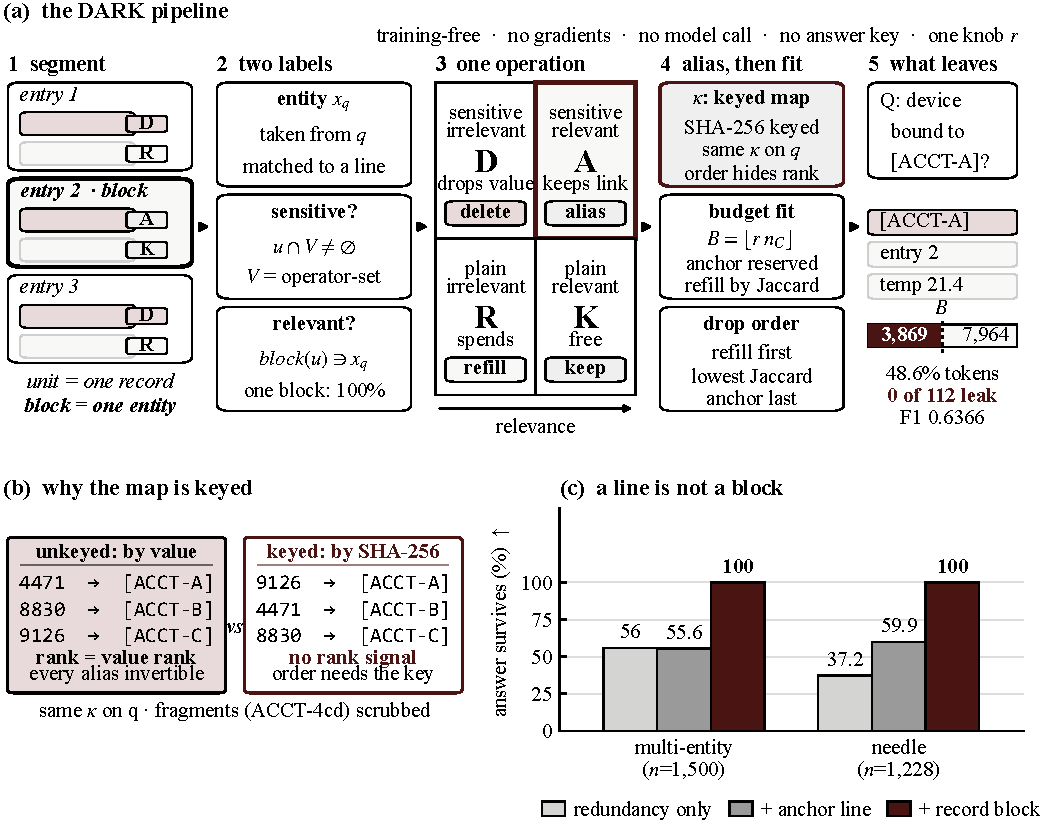
\includegraphics[width=\textwidth]{figures/fig_method.pdf}
\caption{The \textsc{DARK} pipeline. (a) Five stages, all deterministic and model-free.
(1)~Units are lines, grouped into per-entity blocks.
(2)~The question names an entity $x_q$, matched to a line; sensitivity comes from the
protected set $V$ the operator holds, relevance from whether the block contains $x_q$---no
answer key and no model call enters either.
(3)~The pair selects one operation; only the alias cell keeps the value out and the referent
in.
(4)~A keyed map $\kappa$ aliases the protected values and is applied to the question as well;
the entity block is never dropped, and the rest is fitted to $B=\lfloor r\,n_C\rfloor$ in the
stated drop order, refill admitted by decreasing redundancy.
(5)~A real 112-case run: $3{,}869$ tokens against $7{,}964$, no protected value in any
prompt, F1 $0.6366$.
(b)~Why the alias map is keyed. Alias letters handed out in value order are invertible from
their rank alone; deriving the order from a key removes that signal, and the question is
rewritten through the same map so the two halves still agree.
(c)~Protecting the anchor \emph{line} does not close the gap; protecting the \emph{block}
does. Bars give the fraction of the $2{,}728$ cases in which the answer-bearing record
survives.}
\label{fig:pipeline}
\end{figure*}

\begin{algorithm}[t]
\caption{\textsc{DARK} prompt construction}
\label{alg:dark}
\begin{algorithmic}[1]
\Require excerpt $C$, question $q$, budget ratio $r$, protected values $V$
\State $U \gets \textsc{Split}(C)$
\State $A \gets \{u \in U : u \text{ mentions } e^\star(q)\}$
\State $A \gets \textsc{RecordBlock}(U, A)$ \Comment{if markers exist}
\ForAll{$u \in U$}
  \If{$u \in A$}
     \If{$u$ is sensitive} \State alias($u$) \Comment{sensitive and relevant}
     \Else{} \State keep($u$) \Comment{relevant only}
     \EndIf
  \ElsIf{$u$ is sensitive}
     \State delete($u$) \Comment{sensitive and irrelevant}
  \Else{} \State mark $u$ as refill
  \EndIf
\EndFor
\State $P \gets \textsc{Fit}(\text{kept} \cup \text{aliased}, \text{refill}, B)$
       \Comment{hard $B$; degrade, not fail}
\State $q' \gets \textsc{AliasQuestion}(q)$ with the same map
\State \Return $(q', P)$
\end{algorithmic}
\end{algorithm}

\subsection{Relevance from the question}

The relevance label decides which region must survive and which may be spent on the budget.
We use one signal: the region that mentions the entity the question names.
The signal takes two forms in our excerpts.

\paragraph{Record blocks.}
When the excerpt is segmented into blocks headed by a record marker, the whole block that
contains the anchor mention is relevant. This is the common case for log-shaped benchmarks: the
benchmark's own annotation places the reference answer inside the same block as the anchor
mention in every one of its cases (Table~\ref{tab:dataset}). A rule defined on blocks therefore keeps the answer
without inspecting it.

\paragraph{Sentence windows.}
LongBench-style passages carry no block markers. There the relevant region is the anchor
sentence plus one sentence on each side: five units, about $2.3\%$ of the budget in our
measurements. The window is a fallback, not the main mechanism, and
Section~\ref{sec:analysis} reports where it suffices and where it does not.

\paragraph{No answer key.}
A natural implementation of a relevance label is an oracle: mark the unit that contains the
reference answer and deprioritise it last when dropping units. That implementation is not
deployable, and it changes what the method is. We avoid it, and
Section~\ref{sec:analysis} measures how much a pipeline gains from having it, so that the
comparison against an oracle-assisted pipeline is explicit rather than implicit.

\subsection{The four operations and the rewritten question}

Sensitivity is a property of the unit given $V$: a unit is sensitive when it contains a
protected value. Crossing the two labels gives four cells, and each cell receives the
operation that lets the reader resolve the question while the value stays out of the prompt.

\paragraph{Sensitive and relevant: alias (\textbf{A}).}
The unit remains in the context, and each of its protected values is replaced by a stable
alias from a per-run mapping, so that repeated mentions of one entity receive one token.
This cell is where we depart from prior practice. Redaction, the standard primitive, gives
the same concealment but removes the referent. Keeping the unit and renaming its values
preserves the association between the entity and its attributes while satisfying the
constraint on $V$. Section~\ref{sec:analysis} reports the cost of replacing this operation by
deletion: $0.1795$ F1 points overall and $0.3273$ on multi-entity cases.

\paragraph{Sensitive and irrelevant: delete (\textbf{D}).}
The unit holds a protected value that no question component refers to. It contributes
nothing to the answer, so it is removed rather than aliased. This is the only cell in which a
protected value disappears from the prompt entirely.

\paragraph{Relevant and insensitive: keep (\textbf{K}).}
The unit bears on the question and holds nothing that must be hidden, so it is kept verbatim.

\paragraph{Irrelevant and insensitive: refill (\textbf{R}).}
Remaining units hold no protected value and lie outside the relevant region. They compete
for whatever budget is left, ordered by the redundancy score of
Section~\ref{sec:method-budget}.


Aliasing the context alone produces a prompt whose two halves use different names for the
same entity: the context refers to \texttt{[ACCOUNT-A]} while the question still names
\texttt{ACCT-4cd02ed8fb3a}. The reader cannot connect the two, and a string-presence metric
reports the entity as preserved while the task is destroyed. We therefore rewrite the
question with the same map, so that every mention of the queried entity carries the alias
used for it inside the context. The object handed to the model is the pair $(q',P)$, and both
halves are written with one map. Section~\ref{sec:analysis} measures the contribution of
this step.

The alias assignment also determines whether a reader can invert the map by rank. We fix it
per run from a keyed permutation instead of by value order; an unkeyed assignment lets an
adversary who knows the value set recover every alias from its rank alone. All reported
numbers use the keyed assignment.

\subsection{Budget accounting}
\label{sec:method-budget}

The budget is $B=\lceil r\cdot n_C\rceil$, and it is enforced rather than approximated. The
surviving set is assembled greedily and then trimmed against the \emph{actual} concatenated
text, because the separator between units costs tokens: a sum of per-unit token counts is a
lower bound on the length of the joined prompt. When the trimmed set still exceeds $B$,
units are discarded in a fixed priority---refill first, then non-anchor relevant units, then
anchor units---so that the pipeline degrades instead of failing. Every budget arm reported in
this paper has zero overshoot.

Refill ordering uses a model-free redundancy score: for unit $u_i$, the maximum Jaccard
similarity between its token set and that of any other unit. Candidates are visited in
\emph{increasing} redundancy, which keeps the repetitive records.

That direction deserves comment, because it inverts the usual reading of the score. Visiting
units in decreasing redundancy and excluding them is the principled interpretation of a
redundancy measure, and it is what a standard budget-fitting routine does. Here it is the
wrong choice: the answer-bearing record is frequently the most redundant unit, because the
answer value repeats across distractors. Section~\ref{sec:analysis} reports both variants
and the $0.6567$-point difference they produce on the two-hop benchmark. We state the choice
as an empirical regularity with a stated mechanism, not as a consequence of the definition.
